\problemname{Gem Machine
}

Lucy is working on an alien computer chip. The chip can be described by a string $S$ of length $N$. The string contains $A$ types of letters. Since $A$ is at most 26, they are denoted by the first $A$ letters of the English alphabet.

The chip takes a bracket string of length $N$ as input and produces a valuable gem as output. A bracket string comprises only the letters ``\texttt{(}'' and ``\texttt{)}'' and must be properly nested. Every opening bracket is paired with its closing bracket.

The value of the gem is the product of bracket pair values. The value of a bracket pair is $V_{S_i, S_j}$ where $i,j$ are the indexes of the opening and closing brackets respectively and $S_i, S_j$ are the letters at those indexes in $S$.

The overall value of the chip to Lucy is the sum over all the values of the gems it can produce. This is because it will only produce an output gem once for each valid bracket string.

For example, if $S$ = \texttt{ABCACB} and $V$ is the matrix in the top-left corner of the image, there are exactly 5 bracket strings of length 6. The 5 gems produced (values of 112, 36, 48, 84, and 48) are shown in the image.

\begin{center}
 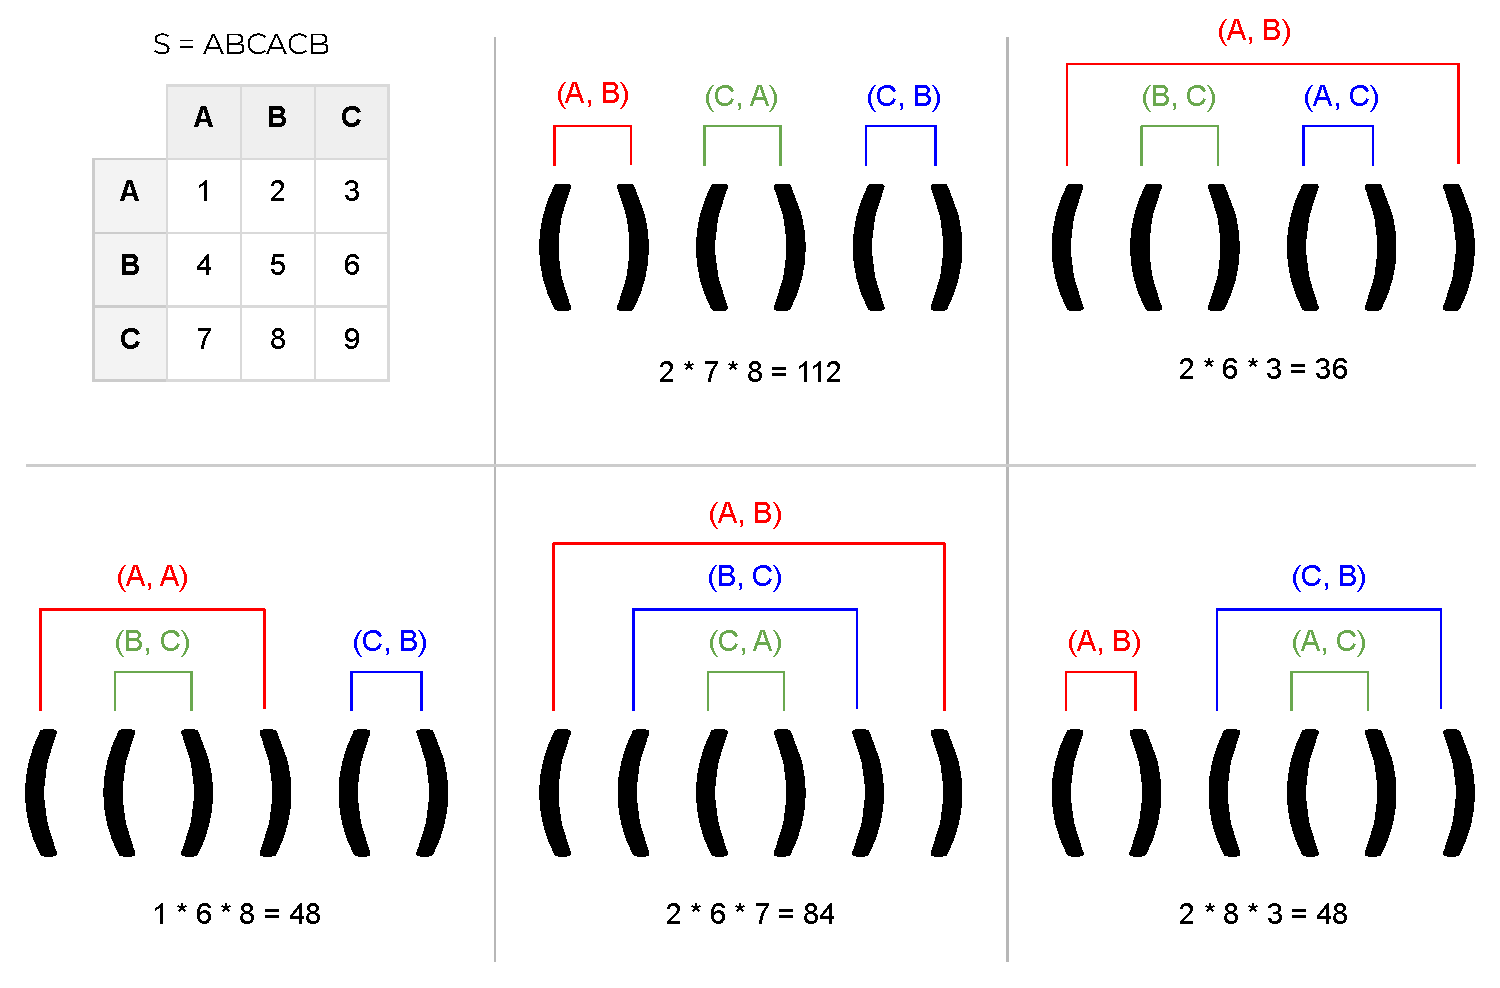
\includegraphics[width=\textwidth]{Brackets}
\end{center}

Lucy has figured out a way to modify exactly one letter in the string $S$. Your job is to write a program to determine for each combination of index and letter, what the overall value of the chip would be if Lucy modified the chip so that it had that letter at that index. It is possible that some of these modifications do not change $S$.


\section*{Input}

The first line of input contains two integers, $N$~($2 \leq N \leq 750$) and $A$~($1 \leq A \leq 26$), which are the length of the string describing the chip and the number of letters in the alphabet respectively. The next line contains the string $S$, which is of length $N$ and from an alphabet consisting of the first $A$ letters of the alphabet. It is guaranteed that $N$ is even.

The next $A$ lines describe the letter pair value matrix $V$. Each line contains $A$ integers each in the inclusive range from 1 to $1\,000$. The $j$th integer on the $i$th line is the value of a pairing between the $i$th letter of the alphabet and the $j$th letter of the alphabet.


\section*{Output}

Display $N \times A$ lines. These lines can be divided into blocks of $A$. The $j$th line in the $i$th block is the value of the chip if the $i$th index in the string were modified to the $j$th letter of the alphabet. Since these values can be large, display each of them modulo $10^9+7$.
